%tex-main
%%%%%%%%%%%%%%%%%%%%%%%%%%%%%%%%%%%%%%%%%%%%%%%%%%%%%%%%%%%%%%%%%%%%%
%% This is a (brief) model paper for submission to the RSC using
%% standard LaTeX packages
%%%%%%%%%%%%%%%%%%%%%%%%%%%%%%%%%%%%%%%%%%%%%%%%%%%%%%%%%%%%%%%%%%%%%


%%%%%%%%%%%%%%%%%%%%%%%%%%%%%%%%%%%%%%%%%%%%%%%%%%%%%%%%%%%%%%%%%%%%%
% Document Formating options 
%%%%%%%%%%%%%%%%%%%%%%%%%%%%%%%%%%%%%%%%%%%%%%%%%%%%%%%%%%%%%%%%%%%%%
% Document Classes 
%\documentclass[journal=jpcafh,manuscript=article,email=false]{achemso}
\documentclass[a4paper,12pt]{article}

% Margins 
\usepackage{geometry} % to change the page dimensions
\geometry{margin=1in} % for example, change the margins to 1 inches all round

% Fonts 
\usepackage[T1]{fontenc} % Modern font encoding
\usepackage{helvet}      % Helvetica font for sans serif
\usepackage{mathptmx}    % Times font ("Word-like")
\usepackage{amsmath}     % Math font 
\usepackage{amssymb}
\usepackage{mathrsfs}

% Spacing 
\usepackage{setspace}    % For double-spacing
\AtBeginDocument{\doublespacing}

% Figures 
\usepackage{float}       % For creating charts, graphs and schemes
\newfloat{chart}{htbp}{loc}
\newfloat{graph}{htbp}{loh}
\newfloat{scheme}{htbp}{los}

% Pictures 
\usepackage{graphicx}    % Embed graphics 
%\graphicspath{./pics/}

% Tables
\usepackage[english]{babel}
\usepackage{array}

% Captions 
\usepackage{subcaption}  % Sub captions ( Table footnotes) 

% Bibliography
\usepackage{rsc}         % Loads natbib, etc

% Sections 
\usepackage{outlines}    % For making outlines 
\usepackage[normalem]{ulem} % For strikethroughs on outline

% Listing 
\usepackage{enumitem}    % Changing the enumerate labels 
\setenumerate[1]{label=\Roman*.}
\setenumerate[2]{label=\Alph*.}
\setenumerate[3]{label=\roman*.}
\setenumerate[4]{label=\alph*.}
%\setlist[enumerate,1]{label=\Roman*}
%\setlist[enumerate,2]{label=\Alph*}

% MISC
\usepackage{cancel}      % For drawing Cancel Out arrows 
\usepackage{pdfpages}  % including the coversheet as a pdf
% Docs http://ctan.mirrors.hoobly.com/macros/latex/contrib/cancel/cancel.pdf

%%%%%%%%%%%%%%%%%%%%%%%%%%%%%%%%%%%%%%%%%%%%%%%%%%%%%%%%%%%%%%%%%%%%%
% Customized Definitions 
%%%%%%%%%%%%%%%%%%%%%%%%%%%%%%%%%%%%%%%%%%%%%%%%%%%%%%%%%%%%%%%%%%%%%
% Math 
\def\ket#1{| #1 \rangle}        %| >
\def\bra#1{\langle#1 |}         %< |
%\def\bm#1{\mbox{\boldmath$#1$}}
\def\bm#1{\mathbf{#1}}
\def\linresp#1#2{\langle\langle#1;#2\rangle\rangle}
\def\quadresp#1#2#3{\langle\langle#1;#2;#3\rangle\rangle}
\def\degrees{deg dm$^{-1}$ (g/mL)$^{-1}$}
\def\optrot{$[\alpha]$}
\def\crt#1{a_{#1}^{\dagger}}    % Creation operator
\def\ann#1{a_{#1}^{\ }}         % annihilation operator 
\def\cgs{($10^{-40}$ cgs)}      % units 
\def\selfolap#1{\langle#1|#1\rangle} % <i|i>
\def\olap#1#2{\langle#1|#2\rangle} %<i|j>
%%%%%%%%%%%%%%%%%%%%%%%%%%%%%%%%%%%%%%%%%%%%%%%%%%%%%%%%%%%%%%%%%%%%%
% Title page 
%%%%%%%%%%%%%%%%%%%%%%%%%%%%%%%%%%%%%%%%%%%%%%%%%%%%%%%%%%%%%%%%%%%%%
%\author{Karl M Pierce \thanks{%
%    Department of Chemistry, Virginia Tech, Blacksburg, Virginia 24061, U.S.A.
%    E-mail: \texttt{kmp5@vt.edu}
%  }
%}
%\title{CHEM 5914 Literature Review and Research Plan -COVERSHEET- Fall 2016}

%%%%%%%%%%%%%%%%%%%%%%%%%%%%%%%%%%%%%%%%%%%%%%%%%%%%%%%%%%%%%%%%%%%%%
%%%%%%%%%%%%%%%%%%%%%%%%%%%%%%%%%%%%%%%%%%%%%%%%%%%%%%%%%%%%%%%%%%%%%
%%%%%%%%%%%%%%%%%%%%%%%%%%%%%%%%%%%%%%%%%%%%%%%%%%%%%%%%%%%%%%%%%%%%%

\begin{document}
%\sloppy
%\maketitle
\singlespacing
\thispagestyle{empty}
%%outline-coversheet.tex

\begin{table}
\centering
{\bf CHEM 5914 Literature Review and Research Plan - COVER SHEET - Fall 2016} \\~\\
\renewcommand{\arraystretch}{1.5}
\begin{tabular}{|l|l|}
    \hline
    {\bf Student's Name} & Kirk C Pearce \\
    \hline
    {\bf Review Title} & \multicolumn{1}{m{10cm}|}{Advanced Quantum Mechanical Simulations of Vibrational Circular Dichroism Spectra} \\
    \hline
    {\bf Student's Email Address} & kcpearce@vt.edu \\
    \hline
    {\bf Date Submitted} & \today \\
    \hline
    {\bf Response Deadline} & December 12, 2016 \\
    \hline
\end{tabular}

\vspace{10mm}

\begin{tabular}{|c|l|}
    \hline
    & {\bf Outline.} Submit to the Research Director only. No specific response deadline. \\
    \hline
    & {\bf Preliminary Draft.} Submit to Research Director only. Response needed by 10/17/16. \\
    \hline
    & {\bf First Draft.} Submit to Advisory Committee. Responses needed by 11/14/16. \\
    \hline
    X & {\bf Final Draft.} Submit to Advisory Committee. Responses needed 12/12/16. \\
    \hline
\end{tabular}

\vspace{10mm}

\begin{tabular}{|c|c|c|c|}
    \hline
    {\bf Function} & {\bf Name} & {\bf Department} & {\bf Email} \\
    \hline
    Chair & T. Daniel Crawford & CHEM & crawdad@vt.edu \\
    \hline
    Member & Edward Valeev & CHEM & valeev76@vt.edu \\
    \hline
    Member & Nicholas Mayhall & CHEM & nmayhall@vt.edu \\
    \hline
    Member & Diego Troya & CHEM & troya@vt.edu \\
    \hline
\end{tabular}
\end{table}
\begin{singlespacing}
\noindent
{\bf Honor Pledge.} Turning in any document for CHEM 5914 constitutes a pledge to conform to the policies and procedures of the Virginia Tech Graduate Honor System. \\~\\
{\bf Faculty Instructions} are available on the CHEM Grad Program site in the Literature Review folder.
\end{singlespacing}





%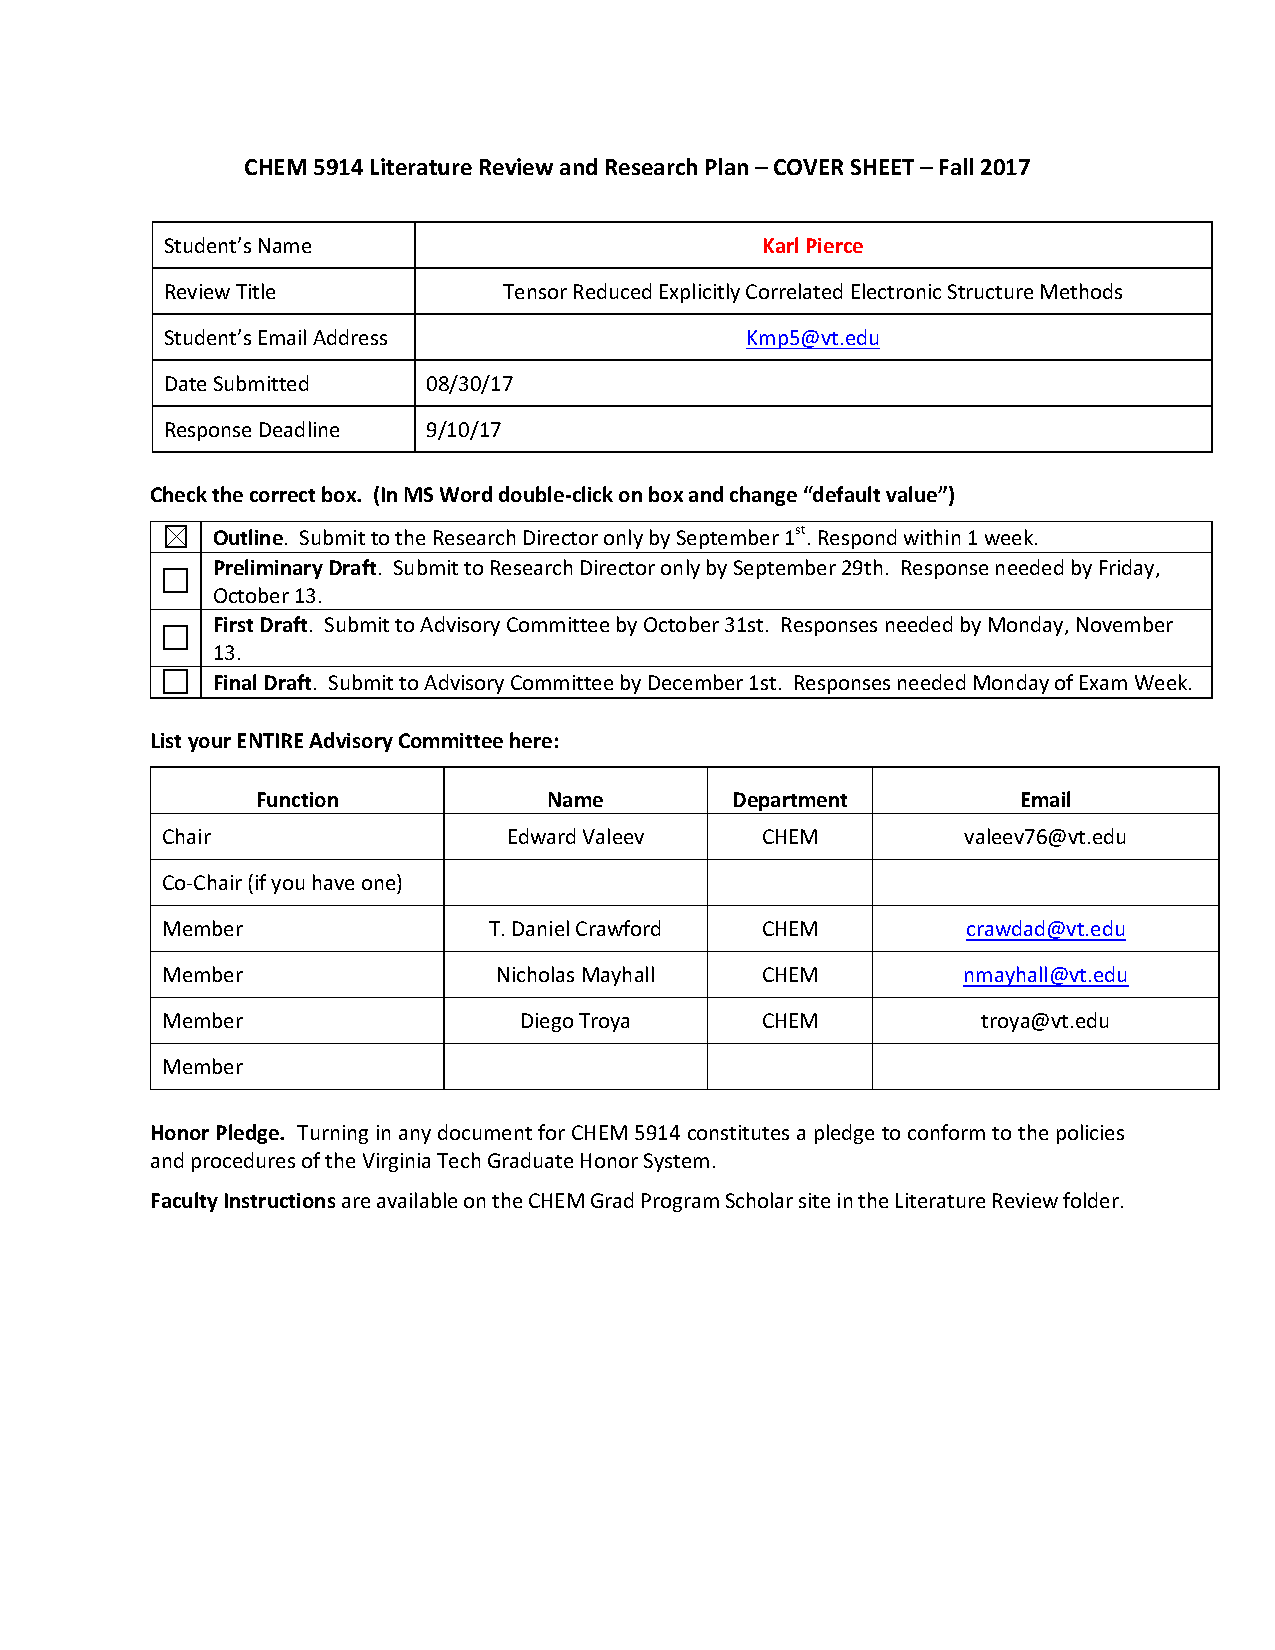
\includepdf[pages={1}]{coversheets/karl_outline-coversheet.pdf}
%%outline.tex

\begin{outline}[enumerate]
    \1 Introduction
        \2 Big picture of analytic derivatives
            \3 Usefulness in quantum chemical calculations
                \4 Properties of interest to all chemists
            \3 Advantages of analytic versus. numerical differentiation
                \4 Numerical accuracy (obviously)
                \4 Increased computational efficiency
            \3 Disadvantages
                \4 Computational cost with higher order derivatives
    \1 \sout{Electronic Structure Theory}
        \2 \sout{Schr\"{o}dinger Equation}
        \2 \sout{Hartree-Fock Theory}
            \3 \sout{Single Determinant Representation minimized with constraint that spin orbitals remain orthonormal}
            \3 \sout{Shortcomings - Mean field approximation (no electron correlation energy)}
        \2 \sout{M{\o}ller-Plesset Perturbation Theory}
            \3 \sout{Treat electron correlation as perturbation to the HF SCF solution}
        \2 \sout{Configuration Interaction}
            \3 \sout{Linear combination of determinants}
            \3 \sout{Variational, but not size consistent}
        \2 \sout{Coupled Cluster Theory}
            \3 \sout{Exponential form of the wave function}
            \3 \sout{Size Consistent, but no variational}
    \1 Optical Response
        \2 Response Theory
            \3 Exact Response
            \3 Linear Response
            \3 Quadratic and Higher Order Response
        \2 Properties
    \1 Analytical Gradient Theory
        \2 Wigner's $2N + 1$ Rule
        \2 First Derivatives
            \3 Derivations
            \3 Associated Properties
        \2 Second Derivatives
            \3 Derivations
            \3 Associated Properties
    \1 Proposed Plan of Study
        \2 Implementation
        \2 Calculation of properties
            \3 CC Simulations of Vibrational Circular Dichroism (VCD) Spectra
            \3 CC Simulations of Magnetic Circular Dichroism (MCD) Spectra
            \3 Non-linear Optical Properties (hyperpolarizabilities)
\end{outline}


\doublespacing
\newpage
%\thispagestyle{empty}
%%outline.tex

\begin{outline}[enumerate]
    \1 Introduction
        \2 Big picture of analytic derivatives
            \3 Usefulness in quantum chemical calculations
                \4 Properties of interest to all chemists
            \3 Advantages of analytic versus. numerical differentiation
                \4 Numerical accuracy (obviously)
                \4 Increased computational efficiency
            \3 Disadvantages
                \4 Computational cost with higher order derivatives
    \1 \sout{Electronic Structure Theory}
        \2 \sout{Schr\"{o}dinger Equation}
        \2 \sout{Hartree-Fock Theory}
            \3 \sout{Single Determinant Representation minimized with constraint that spin orbitals remain orthonormal}
            \3 \sout{Shortcomings - Mean field approximation (no electron correlation energy)}
        \2 \sout{M{\o}ller-Plesset Perturbation Theory}
            \3 \sout{Treat electron correlation as perturbation to the HF SCF solution}
        \2 \sout{Configuration Interaction}
            \3 \sout{Linear combination of determinants}
            \3 \sout{Variational, but not size consistent}
        \2 \sout{Coupled Cluster Theory}
            \3 \sout{Exponential form of the wave function}
            \3 \sout{Size Consistent, but no variational}
    \1 Optical Response
        \2 Response Theory
            \3 Exact Response
            \3 Linear Response
            \3 Quadratic and Higher Order Response
        \2 Properties
    \1 Analytical Gradient Theory
        \2 Wigner's $2N + 1$ Rule
        \2 First Derivatives
            \3 Derivations
            \3 Associated Properties
        \2 Second Derivatives
            \3 Derivations
            \3 Associated Properties
    \1 Proposed Plan of Study
        \2 Implementation
        \2 Calculation of properties
            \3 CC Simulations of Vibrational Circular Dichroism (VCD) Spectra
            \3 CC Simulations of Magnetic Circular Dichroism (MCD) Spectra
            \3 Non-linear Optical Properties (hyperpolarizabilities)
\end{outline}


%\newpage
%introduction.tex%
% Introduction %

\section{Introduction}
%The goal of theoretical chemistry is to further develop mathematics and computational algorithms to predict the accurate properties of chemical systems using the quantum mechanical nature of electrons.  
A grand challenge of theoretical chemistry is to be able to predict accurate properties of chemical systems from the first principles of quantum mechanics. This challenge has many front:  solving increasingly large systems at low cost, predicting chemical properties and finding transition structures to name a few. The electronic and nuclear structure of a chemical system is described by a many body differential equation using Hamiltonian mechanics, known as the Schr{\"o}dinger.  Solving this equation, analytically, in its raw form for non-trivial systems is too difficult. To model chemical systems, therefore, requires mathematical approximations starting from the first principles of quantum mechanics which can accurately approximate solutions to the Schr{\"o}dinger equation.  There exists a number of approximate methods such as Hartree Fock, coupled cluster, and density functional theory which calculate approximate solutions in a balance between computational effort and time, accuracy and chemical system size.
%Therefore, to model chemical systems, physics casts them into a many-body integro-differential equation known as the many-body Schr{\"o}dinger equation.
%The challenge comes from the rigorous mathematics 
%Achieving this goal will push computational analysis to the forefront of investigative research in chemistry reducing the time required to find a chemical for a specific application.  To successfully predict properties of chemicals and reactions, accuracy to an extremely small degree is required in computational chemistry\cite{Shavitt1977}
%Accuracy to an extremely small degree is important to correctly predict the small energy differences in electronic states or different geometries.
%Therefore, it is the task of theoretical chemistry is to provide an approximate framework which preserves the physical nature and accuracy of the exact model. 
%There exists a number of methods applicable to different systems depending on the user's interest to balance computational effort and time, accuracy, and chemical system size. 

%The gold standard in computational chemistry  the coupled cluster methods which are typically used to calculate ground state calculations but require the most computational resources and time. 
Hartree-Fock theory is a mean field approximation which provides a foundation to electronic correlation methods. Hartree-Fock thoery's perturbation based extensions, such as M{\/o}ller-Plesset theory, can be used to calculate electron correlation of molecules with around 100 atoms.  The coupled cluster methods, which are sometimes referred to as the gold standard of electronic structure calculations for their ability to calculate accurate electron correlation energy, require the most computational resources restricting it's calculation ability to molecules with 20-30 atoms. The goal of this research expand the scope of these methods through understanding and manipulation of their computational storage objects, tensors.   %are typically used to calculate energy of molecules with 20-30 atoms.
%Hartree-Fock and its perturbation based extensions such as M{\/o}ller-Plesset methods can recover some electron correlation and can be extended to molecules with around 100 atoms. Other methods such as density functional theory and semi-empirical methods based on classical mechanics can solve even larger molecules though their accuracy can be poor. Other methods such as density functional theory based on classical mechanics can solve even larger molecules though their accuracy can be poor.

In the computation of ab initio quantum mechanics, tensor storage, mutation and contraction are major bottlenecks. The term {\em curse of dimensionality}, first introduced by Bellman\cite{Chen2009} in the field of dynamic programming, refers to the exponential growth in operations required to estimate a function at some accuracy as the number of inputs increases. Using standard, non-decomposed, tensors in the formulation of quantum chemistry calculations is sub-optimal and falls victim to the curse of dimensionality.  Quantum chemists has developed methods which take advantage mathematical tensor structure and the physics which describes the data stored.  Methods such as 
%exponential increase in number of operations required to estimate a function at some accuracy as the number of inputs
%In the formulation of methods described above a major bottleneck is 
%Computational analysis using any one of these methods requires the storage and computation of many index vectors known as tensors.  Tensor storage, manipulation and contraction make up the majority of the bottleneck in the calculation of ab initio quantum chemistry.  In the world of mathematics this is known as the curse of dimensionality.  Though it also known that as dimensionality of tensor storage increases so does sparsity in the full representation of such tensors.  Quantum chemistry has developed methods in order to take advantage of the underlying structure of these tensors, such as projected atomic orbitals, pair natural orbitals and density fitting.  In general these methods reduce computational effort by arbitrarily reducing dimension using some canonical matrix decomposition.  The area of utilizing tensor decomposition in the realm of these physical approximations is sparsely investigated with only the recent introduction of tensor hypercontraction.  Using fast tensor decomposition of physical variables over modern computational architectures can provide data compression without loss of information.  Additionally, as theoretical chemistry pushes to calculate systems to analytical levels of accuracy, such as introduction of explicitly correlated methods, algorithms with extremely large computational scaling factors have developed.  Utilizing the form of tensor decompositions new algorithms can be developed which reduce exponential scaling factors by separating subspaces spanned in the tensor space.

%while reducing mathematical complexity
\input{theoretical/karl_theoretical.tex}
\section{Tensor Algebra Methods to Reduce Computational Complexity in Quantum Chemistry}
	A tensor is a multidimensional array; an N-th order tensor is an element of the tensor product of N vector spaces.
	A first order tensor is an array, a second order tensor is a matrix and tensor of order three or higher is referred to as a higher-order tensor.\cite{Kolda2008}. Tensors are naturally applied to single reference quantum mechanics: operators such as \textbf{F} can be expressed in terms of two electron coordinate products and form second order tensors while other operators and amplitudes such as the coulomb repulsion operator, $\hat{J}$, and the cluster operator amplitudes, $t^{ij\dots}_{ab\dots}$, can be expressed as higher-order tensor. Using tensor's as storage devices creates a problem, known as the "curse of dimensionality", where storage and computational processing required to solve a problem scale exponentially with dimension.
	%This extension therefore means as number of electrons increase, there is an exponential increase in the amount of storage and computational processing required to solve a given problem. This problem is referred to as the "curse of dimensionality" %find a curse of dimensionality paper!%
	To overcome this curse requires one to discover the underlying structure in ones data allowing one to reduce storage requirements and to redesign algorithms to scale with the structure of the data.

	The goal of any tensor decomposition is to reduce the complexity of a tensor via the underlying form of ones data. The result of a tensor decomposition provide information on the relative importance and weighting of individual vector spaces. Direct methods to compute second order, matrix decompositions such as the singular value (SVD), lower-upper (LU), and Jordan decomposition, have been around for quite some time. Though, interests to decompose higher order tensors didn't develop until 1927 with Hitchcock's idea of a tensor to be a polyadic sum of products\cite{Hitchcock1928,Hitchcock1927} and later Cattells's idea of a multi-way model in 1944\cite{Cattell1944,Cattell1952}. These ideas would later be used to develop canonical product(CP) (CANDECOMP/PARAFAC canonical decomposition / parallel factor decomposition) \cite{Carroll1970,Harshman1970} and Tucker decompositions\cite{Tucker1966}. In order to apply ab initio quantum mechanics to larger systems and circumvent the "curse of dimensionality" it is necessary to take advantage of matrix and higher order tensor decomposition approximations and to redesign canonical algorithms using tensors in decomposed form. To follow are theoretical chemist's current tools to approximate and reduce the complexity of large systems while preserving accuracy.
	\subsection{Cholesky Decomposition}
		The Cholesky decomposition (CD) was first applied to quantum chemistry and specifically the two electron integral (TEI) tensor in 1977 by Beeble and Linderberg\cite{Beebe1977} when the authors realized that, coupled with the positive definite nature of the integrals values, one could to reorder the higher-order tensor into a lower order object and perform a matrix decomposition. What makes the CD special is that it can remove small and zero eigenvalues without calculating the entire matrix, providing computational savings. CD has been in conjunction with two electron geminal implementation, derivative integrals and more recently has been applied to large scale TEI decomposition\cite{Aquilante2011}.

		CD works by using a partial (LU) decomposition of any two electron tensor recast into a symmetric positive definite matrix 
			\begin{equation}
				\begin{aligned}
					\label{eqn:CD}
					M_{\mu\nu, \gamma\sigma} = \int \int \rho_{\mu\nu}(r_1)\hat{M}(r_1,r_2) \rho_{\gamma\sigma} dr_1 dr_2 \equiv (\rho_{\mu\nu}|\rho_{\gamma\sigma})
				\end{aligned}
			\end{equation}
		where $\rho_{\mu\nu} = \phi_\mu\phi_\nu$ is an orbital density product and $\hat{M}(r_1,r_2)$ is some two electron operator. The goal of the CD is to express M as 
		%With the goal of expressing
			\begin{equation}
				M = BB^T
			\end{equation}
		This expression can be approximated to some extent, $\gamma$, with elements of M expressed as%therefore elements of M can be expressed as
			\begin{equation}
				\begin{aligned}
					M_{\mu\nu, \gamma\sigma} \approx \sum_{p=1}^{P} B_{\mu\nu}^P B_{\gamma\sigma}^P &= \sum_{p=1}^{P} (\rho_{\mu\nu}|B_p)(B_p|\rho_{\gamma\sigma})\\
					&= \sum_{pq} (\rho_{\mu\nu}|b_p)(\hat{M}(r_1,r_2)^{-1})_{pq}(b_q|\rho_{\gamma\sigma})
				\end{aligned}
			\end{equation}
		where P is the rank of the decomposition which depends on $\gamma$. A comprehensive CD algorithm is presented by Epifanovsky et al\cite{Epifanovsky2013} which can be used to find optimal Cholesky basis, $b_p$, for a given $\hat{M}(r_1,r_2)$
	\subsection{Density Fitting}
		Density fitting (DF) is an specific application of CD where a canonical optimized Cholesky basis is used to decompose the TEI tensor into two order three tensors. The roots of DF have been grounded in Coulomb\cite{Ten-no1995,Vahtras1993} and Exchange\cite{Weigend2002} fitting in Hartree-Fock and has been applied to MP2\cite{Feyereisen1993}, CCSD(T)\cite{Rendell1994} and even explicitly correlated methods\cite{Manby2003}. The derivation of DF to proceed will be based on equations presented by Werner et al.\cite{Werner2003}. The goal of DF is to decompose the TEI tensor
			\begin{equation}
				\begin{aligned}
			\olap{\mu\gamma}{\nu\sigma} = (\mu\nu|\gamma\sigma) &= \int\frac{\phi_\mu(r_1) \phi_\nu(r_1) \phi_\gamma(r_2)\phi_\sigma(r_2)}{r_{12}} dr_1 dr_2\\
			&= \int \frac{\rho_{\mu\nu}(r_1)\rho_{\gamma\sigma}(r_2)}{r_{12}}dr_1 dr_2
				\end{aligned}
			\end{equation}
		one electron densities, $\rho_{\mu\nu}(r) = \phi_\mu(r) \phi_\nu(r)$, can then be approximated as 
			\begin{equation}
				\bar{\rho}_{\mu\nu}(r) = \sum_A^{N_{\text{fit}}} d^{\mu\nu}_A \chi_A(r)
			\end{equation}
		where $\chi_A(r)$ are fitting basis functions and expansion coefficients, $d^{\mu\nu}_A$, are expressed as %can be found by minimizing the functional 
			%\begin{equation}
			%	\Delta_{\mu\nu} = \int dr_1 \int dr_2 \frac{(\rho_{\mu\nu}(r_1)-\bar{\rho}_{\mu\nu}(r_1)) - (\rho_{\mu\nu}(r_2) - \bar{\rho}_{\mu\nu}(r_2))}{r_{12}}
			%\end{equation}
		%which provides 
			\begin{equation}
				d^{\mu\nu}_B = \sum_B (\mu\nu|A)[J^{-1}]_{AB}
			\end{equation}
		where 
			\begin{equation}
				(\mu\nu|A) = \int dr_1 \int dr_2 \frac{\phi_\mu(r_1)\phi_\nu(r_1)\chi_A(r_2)}{r_{12}}
			\end{equation}
		The term J is chosen to be some metric, here it is defined as the coulomb metric\cite{Dunlap1977,Dunlap1979}
			\begin{equation}
				J_{AB} = \int dr_1 \int dr_2 \frac{\chi_A(r_1) \chi_B(r_2)}{r_{12}}
			\end{equation}
		other metrics have been proposed\cite{Baerends1973} and though they are less accurate, these metrics are computed more quickly than the Coulomb metric.\\
		This allows one to express the TEI as 
			\begin{equation}
				(\mu\nu|\gamma\sigma) = \sum_B d^{\mu\nu}_B (B|\gamma\sigma) = \sum_{AB} (\mu\nu|A)[J^{-1}]_{AB}(B|\gamma\sigma)
			\end{equation}
		transforming $J^{-1} = J^{-1/2}J^{-1/2}$ allows one to store the TEI as two order three tensors, reducing storage requirements from $\mathcal{O}(N^4)$ to $\mathcal{O}(N^2\cdot N_{fit}) \approx \mathcal{O}(N^3)$; $N_{fit}$ typically scales linearly with basis set. Using DF Reduced scaling algorithms to calculate values such as the HF Coulomb term, $\hat{J}$, and AO to MO integral transformations et al have been developed.  %Additionally one finds reduction in computational effort in calculations such as the Coulomb term, $\hat{J}$, in HF and transforming integrals from the AOs to MOs in MP2 calculations.\\
		
		To further reduce %the complexity and storage 
		scaling of DF one can choose to use a subset of the full auxiliary basis. Original construction of subsets was developed using distance based domains. Unfortunately, this led to discontinuities on the potential energy surface. Recently it has been shown that a better auxiliary subset includes, for a given density, $\rho_{\mu_a\nu_b}$, fitting functions on either center $a$ or $b$, $|A_{(ab)})$; %. This method is 
		referred to as concentric atomic density fitting (CADF). This idea combined with localization methods and inclusion of exact semi-diagonal terms has been shown to reduce complexity in the calculation and storage of the coulomb, $\hat{J}$, and exchange term, $\hat{K}$, in HF by Hollman et al\cite{Hollman2014}
	\subsection{Direct Tensor Decomposition methods}
		%In the case of matrices, applications of decomposition methods are straightforward and imply the transformation to some canonical form based on the rank of the matrix. 
		Matrix decomposition methods are straightforward and refer to the transformation to some canonical matrix product representation. 
		The extensions of decompositions to higher order tensors is not simple. The rank of a tensor is defined as the smallest number of rank one tensors that generate the tensor as its sum, where a rank one tensor is defined as
			\begin{equation}
				\mathit{X} = a^{(1)} \otimes a^{(2)} \otimes \dots \otimes a^{(N)}
			\end{equation}
		where
			\begin{equation}
				\begin{aligned}
					\mathit{X} &\in \mathbb{R}^{I_1I_2\dots I_N} \\
					a^{(1)} \in \mathbb{R}^{I_1}, \quad a^{(2)} &\in \mathbb{R}^{I_2}, \quad \dots, \quad a^{(N)} \in \mathbb{R}^{(N)}
				\end{aligned}
			\end{equation}
		and a rank R tensor, $\mathit{U}$, can be defined in either the canonical format (CP)
			\begin{equation}
				\mathit{U} = \sum_{r=1}^R \lambda_r a^{(1)}_r \otimes a^{(2)}_r \otimes \dots \otimes a^{(N)}_r \quad \lambda_r \in \mathbb{R}
			\end{equation}
		where $\lambda$ is the normalization of the normalized vectors $a^{(l)}_i$ and one can then define a factor matrix as 
			\begin{equation}
				A^{(l)} = [a^{(l)}_1,\dots a^{(l)}_r]\quad l\in\{1,2,\dots,N\}
			\end{equation}
		such that 
			\begin{equation}
				A \in \mathbb{R}^{I_l R}
			\end{equation}
	 	%It is not necessary to require each factor matrix have the same rank; thus one can define the Tucker decomposition format (also refered to as the higher order singular value decomposition, HOSVD)
	 	Or $\mathit{U}$ can be defined in the Tucker format (also referred to as the higher order singular value decomposition, HOSVD), where each factor matrix is not required to have the same rank, R,
			\begin{equation}
				\mathit{U} = \sum_{\alpha_1}^{r_1} \dots \sum_{\alpha_N}^{r_N} \beta_{\alpha_1\dots\alpha_N}a_{\alpha_1}^{(1)}\otimes \dots \otimes a_{\alpha_N}^{(N)}
			\end{equation}
		where $\{ a_{\alpha_i}^{(l)}\}$ is a set of $R_l$ orthonormal vectors and $\beta \in \mathbb{R}^{r_1,r_2,\dots r_n}$ is the Tucker core tensor. Figure's 2 and 3 depict diagrammatically the CP and Tucker format
	  \begin{figure}
		\centering
			\begin{minipage}{.5\textwidth}
			  \centering
			  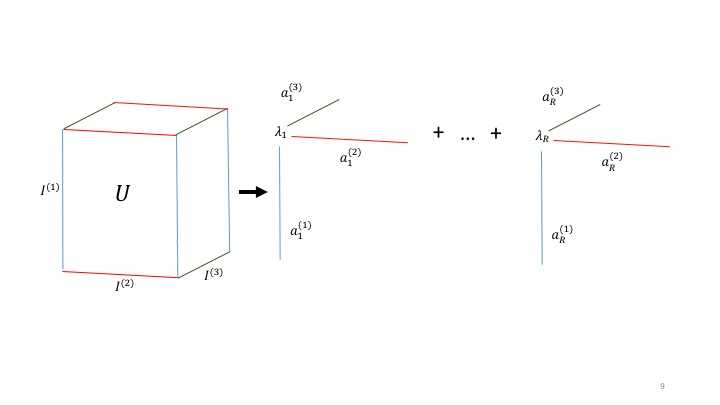
\includegraphics[width=1\linewidth]{./pics/CP_picture.jpg}
			  \captionof{figure}{Representation of CP format}
			  \label{fig:Figure 2}
			\end{minipage}%
			\begin{minipage}{.5\textwidth}
			  \centering
			  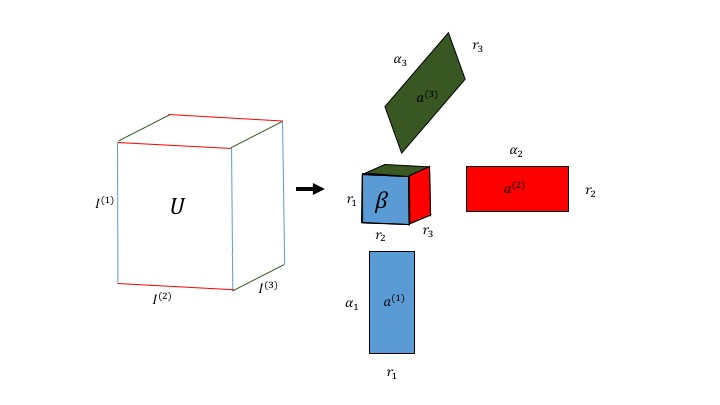
\includegraphics[width=1 \linewidth]{./pics/Tucker_picture.jpg}
			  \captionof{figure}{Representation of Tucker format}
			  \label{fig:Figure 3}
			\end{minipage}
		\end{figure}

	  Unlike matrix decompositions, there are no concise method to calculate the rank of a tensor, solving the rank is an NP hard problem\cite{Hastad1990}. Though there are many schemes which can solve for the approximate rank of a tensor, $\mathit{T}$, by iteratively minimizing a series of non-linear equations\cite{Kolda2008}
	  	\begin{equation}
	  		\begin{aligned}
	  			\|\mathit{T} - \mathit{U}\| < \epsilon
	  		\end{aligned}
	  	\end{equation}
	  where $\mathcal{U}$ is defined using canonical or Tucker format. 

	  Historically, the Tucker decomposition is linked to complete active-space self-consistent field (CASSCF) method\cite{Roos1980}, where the decomposition of excitation amplitudes yields optimized orbitals and the CP decomposition can be linked to full CI\cite{Bell2010} (FCI) where methods such as perfect pairing approach can be considered rank one tensor approximations to the FCI tensor. Applications of the CP decomposition to FCI recently resurfaced\cite{Uemura2012,Bohm2016}. %. The idea of using CP decomposition for FCI has recently resurfaced\cite{Uemura2012,Bohm2016}. 
	  Today, there is an effort to make use of the tensor element sparsity that naturally occurs as dimension increases to decompose tensors in canonical ab initio methods. In work presented by Benedikt et al\cite{Benedikt2011,Benedikt2013,Benedikt2013a,Benedikt2014}, post-HF operator and amplitude tensors are decomposed to compute MP2 and CCD using CP format for example
	  	\begin{equation}
	  		(\mu\nu|\rho\sigma) = \sum_r^R \chi^{(\mu)}_r \otimes \chi^{(\nu)}_r \otimes \chi^{(\rho)}_r \otimes \chi^{(\sigma)}_r
	  	\end{equation}
	  Using this form the authors developed equations to preserve decomposed form and rank. These methods allow for reduced complexity in storage with out significant trade-off in accuracy. In this form efforts to compute a single index contraction between two tensors of order $d$ and $f$ with dimension of each order $N$ decomposed to rank $R_1$ and $R_2$ are reduced from scaling as $\mathcal{O}(N^{d + f -1})$ to $\mathcal{O}(N \cdot R_1 * R_2)$. 
	  %and reduce the computational effort to perform any d-th order tensor contraction from $\mathcal{O}(d)$ to $K \cdot d \cdot R1 \cdot R2$ where K is the number of orbitals, d is the dimension of the tensors, and R1 and R2 are the ranks of each tensor. 
	  Unfortunately, finding the optimal rank and CP decomposition of tensors, such as the TEI, is non-trivial and costly and tensor contractions increases storage requirements, though it is possible to perform decompositions to reduce the contracted tensor rank. Therefore, implementation of CP decomposed post-HF methods are not yet desirable.  Efforts to implement a fast tensor compression algorithm to reduce the effort of computing the CP decomposition will be discussed in the research sections.

	  In work presented by Bell et al\cite{Bell2010} truncated HOSVD is employed to decompose the MP2 method $T_2$ amplitude expression, 
	  	\begin{equation}
	  		T_2(i,a,j,b) = \frac{(ia|jb)}{\epsilon_i + \epsilon_j - \epsilon_a - \epsilon_b}
	  	\end{equation}
	  This author showed that HOSVD could reduce storage of $T_2$ amplitudes for MP2 energy recovery from 85 to 99\%. Additionally, they showed that orbital active spaces obtained through the HOSVD coincide with physical intuition based on how the tensor is unfolded, in the first step of the HOSVD algorithm. Though the HOSVD does have some downsides, first HOSVD alone does not provide an optimal basis in terms of energy recovery it must therefore be coupled with other tensor decompositions and the algorithm to compute the HOSVD scales asymptotically as $\mathcal{O}(N^5)$\cite{Bell2010}.
	\subsection{Tensor Hypercontraction}
		Tensor Hypercontraction (THC) was introduced in 2012 by Hohenstein, Parrish and Martinez\cite{Schutski2017}. THC can be though of as a tensors decompositions applied to a DF decomposition, though in practice a CD or DF is not required. The THC for the TEI for example can be formulated a number of ways. As an example a TCH on a general four index tensor (FIT) will be derived. THC's goal is to recompose the FIT as a connected product of matrices 
			\begin{equation}
				V_{pqrs} \approx W_{p,\alpha} W_{q,\alpha} X_{\alpha\beta} W_{\beta, r} W_{\beta,s}
			\end{equation}
		First the step is to rewrite the FIT as a two index tensor
			\begin{equation}
				V_{pqrs} = V_{pq,rs}
			\end{equation}
		Then using an SVD one can express the two index tensor as
			\begin{equation}
				V_{pq,rs} = U_{pq,\lambda}S_{\lambda,\lambda} V^T_{\lambda, rs}
			\end{equation}
		where $\lambda$ is the rank of the decomposition, $U$ and $V^T$ are unitary matrices and $S$ is the singular value matrix. Here one may choose to use a truncated SVD or CD or DF. The singular values are then rerepresented as $S = S^{1/2} S^{1/2}$ and multiplied into the left and right singular vectors.
			\begin{equation}
				V_{pq,rs} = \tilde{U}_{pq, \lambda} \tilde{V}^T_{\lambda,rs}
			\end{equation}
		If one uses the CD or DF, a matrix roots of the overlap, $J^{1/2}$ of $J_{\lambda,\lambda}$ must be found to using an eigenvalue decomposition or SVD. Next, a CP decomposition is performed on the three index tensors $\tilde{U}$ and $\tilde{V}$
			\begin{equation}
				\begin{aligned}
					\tilde{U}_{pq, \lambda} = W_{p,\alpha} W_{q, \alpha} W_{\alpha, \lambda}\\
					\tilde{V}^T_{\lambda,rs} = W_{\lambda, \beta} W_{\beta, r} W_{\beta, s}
				\end{aligned}
			\end{equation}
		where $\alpha$ and $\beta$ are the rank of the CP decomposition. So far only applications where $\alpha = \beta$ have been studied. Finally the terms $W_{\alpha, \lambda} \text{ and } W_{\lambda, \beta}$ are contracted and one finds
			\begin{equation}
				V_{pqrs} = W_{p, \alpha} W_{q, \alpha} X_{\alpha, \beta} W_{\beta, r} W_{\beta, s}
			\end{equation}
		where
			\begin{equation}
				X_{\alpha, \beta} = W_{\alpha, \lambda} W{\lambda, \beta}
			\end{equation}
		THC has been used in the field to represent the electron interaction potentials in CC2 methods and to decompose the TEI used to calculate CCSD and FCI energies. In work presented by Hummel et al\cite{Hummel2016} using THC the scaling of distinguishable CCD or linearlized CCSD from $\mathcal{O}(N^6)$ to $\mathcal{O}(N^5)$ and in work presented by Schutski et al\cite{Schutski2017}using THC scaling of CCSD was reduced to $\mathcal{O}(N^4)$. Schutski also presents a direct THC method which allows TEI decomposition to scale as $\mathcal{O}(N^5)$ using the SVD or $\mathcal{O}(N^4)$ using a DF scheme while preserving accuracy of \textasciitilde.5 millihartree .
	\subsection{Orbital localization methods}
		A non-obvious method to reduce the complexity of tensors is to define new more compact occupied and unoccupied orbital sets, such is the basis for the projected atomic orbitals (PAO), pair natural orbitals(PNO) and orbital specific virtual (OSV) methods. Conveniently, unitary transformations of the molecular orbital space which do not mix occupied and unoccupied orbitals commute with all observable operators\cite{SzaboAttila1982} and these transformations can be used in orbital localization correlation (LC) methods. There are many developed orbital localization schemes such as Boys and Pipek-Mezey\cite{Boughton1993} among others which are utilized by PNO, PAO and OSV methods. In all the following methods MO are optimized using HF, though other optimizations are possible. Localized occupied MO's (OMO) will be denoted i,j,k and canonical unoccupied MOs (UMO) will be denoted a,b,c, non-canonical UMO's will be denoted r,s,t. All the following methods start by localizing the set of canonical OMO's. Below is a formula to generate a new occupied electron pair specific UMO's 
			\begin{equation}
				\ket{r^{ij}} = \sum_a \ket{a}R^{ij}_{ar}
			\end{equation}
		where $R^{ij}_{ar}$ is a pair specific transformation matrix. Using this occupied electron pair specific UMO one can transform the $T_1$ and $T_2$ amplitudes%This allows one to transform $T_1$ and $T_2$ amplitudes as 
			\begin{equation}
				t^i_a = \sum_{r\in[ii]} R^{ij}_{ar}t^i_r
			\end{equation}
			\begin{equation}
			t^{ij}_{ab} = \sum_{r\in[ij]} R^{ij}_{ar}t^{ij}_{rs}R^{ij}_{bs}
			\end{equation}
		In this format, correlation amplitudes and residual equations can be redefined and if possible reduced using domain approximations based on occupied electron pair distances\cite{Yang2012}.
		The PAO method works by projecting AO basis functions against the UMO's\cite{Pulay1983}
			%\begin{equation}\label{proj_AO}
			%	\ket{\tilde{\phi}_\mu} = \left(1- \sum_{i=1}^{m} \ket{(\chi_i)_L}\bra{(\chi_i)_L} \right) \ket{\phi_\mu} = \sum_{\rho=1}^N \ket{\phi_\rho}\tilde{R}_{\rho\mu}
			%\end{equation}
			%where the expansion coefficient of the projected functions $\tilde{\phi}_\mu$ in AO basis $\{\phi_\mu\}$ is given by 
			%	\begin{equation}
			%		\mathbf{\tilde{R}} = 1 - \mathbf{D} \cdot \mathbf{S}
			%	\end{equation}
			%where \textbf{D} and \textbf{S} are obtained during HF procedure\cite{Hampel1996}
			\begin{equation}
				\ket{r} = \sum_a \ket{a}R_{ar}
			\end{equation}
		where
				\begin{equation}
					R_{ar} = \olap{a}{\phi_r}
				\end{equation}
		This type of localization ensures the unoccupied space be orthogonal to the occupied space, but vectors in the unoccupied space are not orthogonal. PAO implementation has large impact in its implementation in CCSD(T), equation of motion CCSD, and more recently R12 methods by Werner et al\cite{Riplinger2013}. The number of PAOs to obtain accurate recovery of correlation energy (>99\%) grows linearly with size of the basis set per atom and domain sizes are asymptotically independent of molecule size.

		In PNO methods $R^{ij}_{ar}$ is defined by diagonalizing the MP2-like density matrix\cite{Yang2012,Neese2009}
			\begin{equation}
				D^{ij} = \frac{1}{1+\delta_{ij}}(\tilde{T}^{ij}T^{ij} + \tilde{T}^{ij}T^{ij^\dagger})
			\end{equation}
		where
			\begin{equation}
				T^{ij}_{ab} = \frac{\olap{ij}{ab}}{\epsilon_i + \epsilon_j - \epsilon_a - \epsilon_b}
			\end{equation}
			\begin{equation}
				\tilde{T}^{ij}_{ab} = 2T^{ij}_{ab} - T^{ji}_{ab}
			\end{equation}
		such that
			\begin{equation}
				D^{ij}R^{ij}_r = n^{ij}_rR^{ij}_r
			\end{equation}
		where $n^{ij}$ is the natural occupation number. Thus PNOs can be expanded in the basis of UMO or vice versa as
			\begin{equation}
				\ket{r^{ij}} = \sum_a R^{ij}_{ar} \ket{a}
			\end{equation}
			\begin{equation}
				\ket{a} = \sum_r \bar{R}^{ij}_{ar} \ket{r^{ij}}
			\end{equation}
		PNOs for a given pair are orthogonal but PNOs between pairs are non-orthogonal. One can truncate the full set of PNOs using the occupation number as a threshold; it has been found that 30 to 40 PNOs per electron pair can recover 99.9\% of canonical correlation energy for a triple-$\zeta$ basis set. Unfortunately the number of PNOs scales with the number of pairs so the total number of PNOs might still be too large. To compensate one can also truncate the set of [ij] pairs based on a pair MP2 energy threshold. The PNO methods formal scaling is $\mathcal{O}(N^5)$ though the approximations described above among others have allowed for the development of near linear scaling PNOs in CCSD\cite{Riplinger2013}

		More recently Yang et al\cite{Yang2011} has combined the ideas of pair independent PAOs and pair specific PNOs and proposed an OSV method. In this method $R^{ij}_{ar}$ is found by SVD of the diagonal MP2 pair amplitudes. 
			\begin{equation}
				[R^{i\dagger} T^{ij} R^{i}]_{rs} = t^{ii}_r \delta{rs}
			\end{equation}
			\begin{equation}
				\ket{r^i} = \sum_a \ket{a}Q^i_ar
			\end{equation}
		Like PNOs, OSVs of a single OMO are orthogonal but OSVs of different OMO's are non-orthogonal. It has been shown that typically 100 OSVs are required to recover 99.8\% of correlation energy, requiring fewer orbitals than both PNO and OSV methods. Construction of OSVs scales as  $\mathcal{O}(N^4)$
%%gradient.tex%
% Analytic Gradient Theory %

\section{Analytical Gradient Theory}
    There is a deep underlying connection between response theory and gradient theory. In fact, the properties that are calculated with response functions can also be calculated with energy derivatives. Both approaches deal with a system that is subject to some perturbation, however, the difference between the two lies in the nature of the perturbation. Perturbations are often thought of as external electric or magnetic fields, but changes in nuclear coordinates or any other slight change to the system may also be considered to be perturbations. Due to the Fourier transformed perturbation in equation (\ref{eq:FT}), response functions can be used to calculate dynamic properties that depend on the frequency $\omega$ of an external field. Moreover, response functions can also be used to calculate properties generated by a static field by setting $\omega$ equal to zero. On the other hand, derivatives of the energy are used to calculate static field properties because their formulation inherently lacks a frequency dependence. For example, the dynamic polarizability of a molecule due to a frequency-dependent external electric field may be calculated using the linear response function, whereas an induced electric dipole moment (static polarizability) can be calculated using the second derivative of the energy with respect to the external electric field.

    Ultimately, energy derivatives can be calculated numerically or analytically, but analytical differentiation has a few major advantages when compared to numerical differentiation. The first advantage is obviously numerical accuracy. The accuracy of numerical differentiation is highly dependent on the increment size, resulting in errors if the increments are too small or too large, whereas, analytical derivatives avoid approximations and are only limited by numerical precision of the computer. The second advantage to using analytical derivatives is computational efficiency. For example, all analytical first derivatives of the energy with respect to nuclear positions can be calculated with a comparable computational cost to calculating the energy in the first place. An additional advantage to analytic gradients vs. numerical is that you can't use the latter for frequency-dependent properties. The main disadvantage of analytical derivatives stems from the difficulties in implementation, especially with respect to storage requirements and parallelization\cite{Pulay2014}.
\subsection{History}
    The first derivations of HF first and second derivatives was presented by Brato{\v{z}}\cite{Bratoz1958} in 1958, however, it remained unpopular due to its early introduction. 10 years later, Gerratt and Mills\cite{Gerratt1968} proposed the idea of calculated force constants as analytical derivatives of Hellmann-Feynman forces, which ultimately proved to be an unreliable approach. Pulay reintroduced analytical first derivatives in 1969\cite{Pulay1969} suggesting that analytical derivatives should stop at the first derivative, and force constants should be calculated by numerical differentiation of the first derivatives. Pople et al.\cite{Pople1979} were the first to report a practical implementation of second derivatives for HF and MP2, representing the first extension of analytical derivatives to a dynamical electron correlation method. Since, analytical first and second derivatives have been extended to CI\cite{Krishnan1980,Brooks1980}, DFT, and CC at various levels of theory\cite{Scheiner1987,Lee1991,Koch1990a,Gauss1997} made practical through the Z-vector technique\cite{Hoffmann1984}.
\subsection{Wigner's $2N+1$ Rule}
    Regardless of whether response theory or analytical gradient theory is used, certain knowledge about the wave function is necessary in order to calculate certain properties. This is a consequence of the fact that perturbation theory and analytical gradient theory are both subject to Wigner's $2N+1$ rule\cite{Wigner1935}, which states that knowledge of the wave function through $N$th order provides enough information to evaluate the ($2N+1$)th perturbation contributions, or energy derivatives. This means that the zeroth order derivative of the wave function is adequate to determine the first derivative of the energy. A consequence of this is that the computational cost of calculating all nuclear first derivatives is similar to the cost of the energy. Likewise, the first order derivative of the wave function will suffice to calculate the second and third derivatives of the energy. In CC theory, Wigner's $2N+1$ rule applies to the T amplitudes in that knowledge of the T amplitudes through $N$th order is sufficient for the ($2N+1$)th perturbative corrections to the energy. There is an analogous $2N+2$ rule for the $\Lambda$ amplitudes as well\cite{Eriksen2014}. 
\subsection{Associated Properties}
    The calculation of analytical energy derivatives has revolutionized quantum chemistry, making electronic structure calculations accessible and useful for a sizable number of chemists. Table 1 lists some observable quantities and their associated energy derivatives\cite{Pulay1995}. 
    \begin{table}
    \caption {Energy Derivatives and Observables}
    \small
    \begin{center}
        \begin{tabular} {| c | p{13cm} | }
            \hline & \\
            \multicolumn{1}{|c|}{\bfseries Quantity} & \multicolumn{1}{|c|}{\bfseries Observable} \\ & \\
            \hline & \\
            $\frac{\partial E}{\partial R}$ & forces on the nuclei; critical points on the potential energy surface (minima and saddle points) \\ & \\
            $\frac{\partial^2 E}{\partial R_i \partial R_j}$ & force constant, fundamental vibrational frequencies; infrared and Raman spectra; vibrational amplitudes; vibration-rotation couplings \\ & \\
            $\frac{\partial^3 E}{\partial R_i \partial R_j \partial R_k}$ & cubic force constants; anharmonic contributions to vibrational frequencies; anharmonic contributions to vibrational averages \\ & \\
            $\frac{\partial^4 E}{\partial R_i \partial R_j \partial R_k \partial R_l}$ & quartic force constants; anharmonic contributions to vibrational frequencies \\ & \\
            $\frac{\partial E}{\partial F}$ & dipole moment; intermolecular forces \\ & \\
            $\frac{\partial^2 E}{\partial F_\alpha \partial F_\beta}$ & polarizability; intermolecular forces; light scattering \\ & \\
            $\frac{\partial^3 E}{\partial F_\alpha \partial F_\beta \partial F_\gamma}$ & (first) hyperpolarizability; second harmonic generation \\ & \\
            $\frac{\partial^2 E}{\partial R_i \partial F_\alpha}$ & dipole moment derivative; infrared intensities \\ & \\
            $\frac{\partial^3 E}{\partial R_i \partial F_\alpha \partial F_\beta}$ & polarizability derivative; Raman intensity \\ & \\
            $\frac{\partial^3 E}{\partial R_i \partial R_j \partial F_\alpha}$ & electrical anharmonicity, intensities of overtones in the infrared spectrum; vibrationally averaged dipole moments; electric field effect on the harmonic force constants \\ & \\
            $\frac{\partial E}{\partial B}$ & magnetic dipole moment \\ & \\
            $\frac{\partial^2 E}{\partial B_\alpha \partial B_\beta}$ & magnetic susceptibility \\ & \\
            $\frac{\partial^2 E}{\partial B_\alpha \partial \mu_\beta}$ & NMR chemical shielding \\ & \\
            $\frac{\partial^3 E}{\partial R_i \partial F_\alpha \partial B_\alpha}$ & infrared optical rotatory power \\ & \\
            \hline
        \end{tabular} \\
        \bigskip
        \textit{Notation: R: nuclear coordinate; F: electric field; B: magnetic flux density; $\mu_{\beta}$: the $\beta$ component of the magnetic moment.}
    \end{center}
    \end{table}
    While many chemists are only interested in black box calculations that make use of only the simplest energy derivatives (e.g. forces and force constants for geometry optimizations), a wide range of chemical properties can be predicted with significant accuracy using energy derivatives. For example, energy derivatives are essential to calculating magnetic properties such as magnetic dipole moments, NMR spectra, magnetizability, etc.\cite{Pulay2014} 


%\section{Research Plan}
	It is apparent from the literature that operators and amplitude expressions in tensors in quantum chemistry have some compact format that can be taken advantage %of as the dimension of a system increases, ie number of electrons. 
	It is the goal for this research to apply tensor decomposition algorithms, which make use of modern computational architecture, to reduce computational complexity of correlation methods based on MBPT, CC, and CC-R12 methods. 
	%modern computational architecture scaling tensor decomposition algorithms to reduce scaling of correlation methods based on MBPT, CC and CC-R12 methods. 
	%THC is quantum chemistries first step into utilizing the structure of tensor decompositions to reduce storage requirements without arbitrary truncation based on practiced thresholds.
	%CP and Tucker decompositions dissect the character from the full set of vectors which span the tensor space, unlike the truncated SVD or eigenvalue decomposition. 
	CP and Tucker decompositions encode the behavior of every element in a given tensor into a set of factor matrices with reduced storage requirements. 
	%In PNO and OSV methods virtual set domain truncation is based on either a occupation number or the diagonal MP2 amplitude threshold and rank is reduced by removing information.  
	While truncation methods based on an eigenvalue, occupation number, or diagonal MP2 amplitudes discard information deemed unnecessary. Implementing tensor decompositions, instead of these truncation methods, to reduce storage requirements allows for data compression without significantly loss of information. Figure 4 and 5 show how memory requirements of canonical tensors in quantum chemistry, such as the TEIs, can be significantly reduced with little cost in accuracy.
	%Changing these rank reduction methods to tensor decompositions would allow for data compression without loss of information. These new rank reductions methods c assist in the calculation of molecular properties where for example loss of even small valued vectors could have large contributions in derivative based response properties. 

		\begin{figure}
			\centering
				\begin{minipage}{.5\textwidth}
				  \centering
				  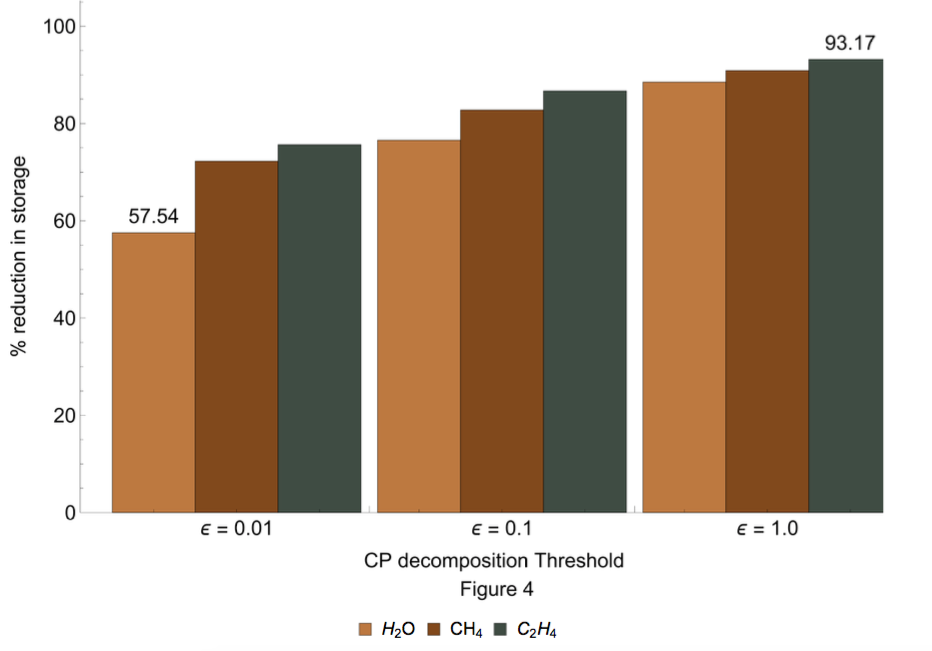
\includegraphics[width=1\linewidth]{./plots/Store}
				  %\captionof{figure}{Reduced storage requirements of TEI after CP decomposition }
				  \label{fig:Figure 4}
				\end{minipage}%
				\begin{minipage}{.5\textwidth}
				  \centering
				  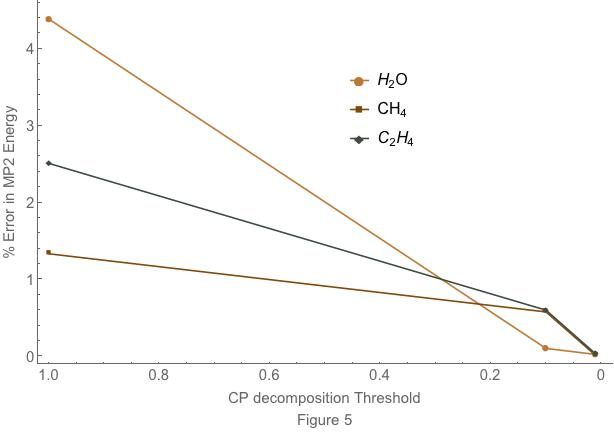
\includegraphics[width=1 \linewidth]{./plots/Energy}
				  \label{fig:Figure 5}
				\end{minipage}
				\caption{Reduced storage requirements of global AO TEI tensor after CP decomposition\\
				\textbf{Figure 5:} MP2 energy calculated using the CP decomposed global AO TEI methods presented by Benedikt et al\cite{Benedikt2011} compared to canonical closed-shell spin-restricted MP2 calculations.\\
				Following Benedikt's implementation the HF orbital energy denominator term was decomposed to a CP threshold of $\epsilon = .01$; Calculations on $\text{H}_2\text{O}$ and $\text{CH}_4$ were performed using a 6-31G* basis and calculations on $\text{C}_2\text{H}_4$ used a 6-31G basis}
		\end{figure}

	In order to reduce the computational demands of computing the CP decomposition modern mathematics turns to tensor compression.  Tensor compression techniques reduce computational bottleneck of large tensor using a smaller proxy tensor, which are then used to approximately the CP decomposition. Original methods to compute a tensor compression used the Tucker decomposition\cite{Bro1998,Lathauwer2000}. However, this approach requires the computation of an expensive singular value decomposition on each mode of a tensor. More recently, mathematicians have found that randomized tensor compression methods can achieve significant computational savings while producing near-optimal approximation quality\cite{Erichson2017}. Application of these compression methods, to tensors which are too either large to store in fast memory or are slow to converge to their optimal rank, will allow for reduced scale tensor algebra methods to be more reasonably applied to single reference quantum chemistry.

	Generally the tools in computational chemistry have limited application, such as CCSD(T) or CCSD-RI, because computational scaling and storage  requirements are unmanageably high.  Work presented by Benedikt et al\cite{Benedikt2011,Benedikt2013,Benedikt2013a,Benedikt2014} is the first step to understanding how to reformulate canonical many-body ab initio quantum mechanic equations into a decomposed tensor algebra framework.  Benedikt's ideas can be extended by work presented by Parrish et al\cite{Parrish2012}.  Using the CP decomposition on a form of DF TEI reduces the storage requirements of integral tensor while tensor algebra expressions reduce the operations required to calculate observables. This idea can be further extended to reduced scaling accurate molecular properties. For example using CADF work presented by Hollman et all\cite{Hollman2014}, one can compute "localized" analytical gradients of the TEIs where, either the gradients are decomposed during their computation or CADF third order tensors are first decomposed then analytical gradient expressions are calculated using tensor algebra expressions.  
	%Though, tensor decomposition methods to compress higher order amplitude expressions has not yet been explored by quantum chemistry. Tensor decompositions will also allow for method development in reduced scaling accurate molecular property investigation, where truncation based approaches can significant influence a property's value.
  %Application of CP decompositions to CADF will decouple electronic indices's from electronic density terms allowing one to calculate more simply HF exchange terms. %Hollman and co-authors CADF method reduced computational cost with less error th 

	In work originally presented by Alm{\"o}f\cite{Almlof1991} and later H{\"a}ser\
	\cite{Haser1992} it has been shown that the AO to MO integral transform step of perturbation methods, such as MP2 \cref{AO2MO}, can be simplified using a Laplace transform of the denominator term
		\begin{equation}\label{LP_MP2}
			D_{ijab} = \frac{1}{\epsilon_i + \epsilon_j - \epsilon_a - \epsilon_b} = \int e^{(\epsilon_i + \epsilon_j - \epsilon_a - \epsilon_b)t}dt
		\end{equation}
	from there the exponential term can be factored into the AO wavefuntion
		\begin{equation}
			\ket{\phi_i} = \ket{\phi_i}e^{-\epsilon_i t/2}
		\end{equation}
		\begin{equation}
			\ket{\phi_a} = \ket{\phi_a}e^{\epsilon_a t/2}
		\end{equation}
	Computationally the integral in \cref{LP_MP2} can be transformed to a finite sum
		\begin{equation}
			E_{MP2} = \sum_\alpha^\tau w_\alpha e_2^\alpha
		\end{equation}
	$e_2^\alpha$ is the weighted integral form of \cref{AO2MO} based on the difference in energy between $\epsilon_i$ or $\epsilon_a$ and $\epsilon_F$ the fermi level.  These integrals can be in AO basis or any non-canonical form.  Using tensor decomposition methods one can optimize the weighting coefficients and calculate more accurate quadrature points.  Laplace transform methods coupled with tensor decompositions to perturbation theories, such as CCSD(T) and CCSD(T)-R12, could reduce the storage and computational complexity of these methods allowing one to compute energy values of increasingly large molecules extremely accurately.
\newpage
\singlespacing
%\bibliographystyle{rsc}
\bibliography{references.bib}
\end{document}
%%%%%%%%%%%%%%%%%%%%%%%%%%%%%%%%%%%%%%%%%%%%%%%%%%%%%%%%%%%%%%%%%%%%%

